\chapter{PARKIBIP: Manual de usuario del sistema}

\section{Instalación de PARKIBIP}

Una vez que se descarga la aplicación PARKIBIP en el teléfono, la instalación de la misma se realiza de manera automática. Así, luego de un proceso de instalación satisfactorio, es preciso ubicar el icono ejecutable de la aplicación descargada, para asegurarse que se encuentra instalada correctamente -ver Fig. \ref{fig:instalation-parkibip}-. 

\begin{figure}[H]
 \centering
 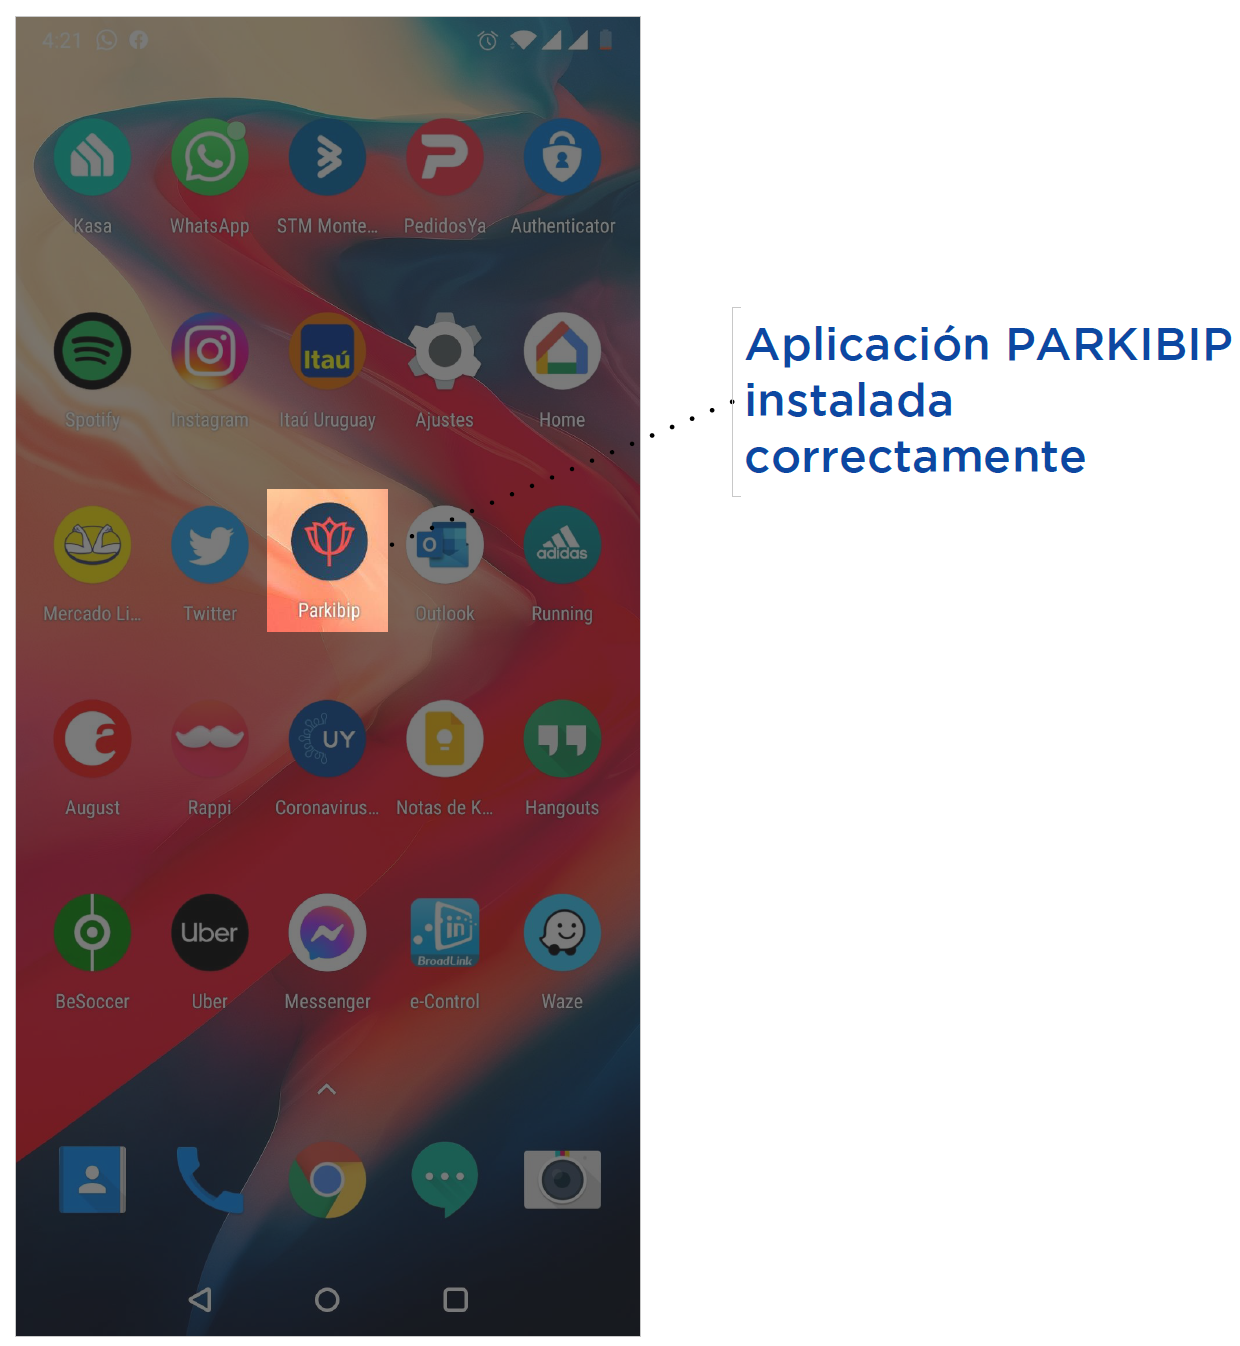
\includegraphics[height=8cm]{TESIS/imagenes/user-manual/manual-instalation.PNG}
 \caption{Icono de la aplicación PARKIBIP en el menú de aplicaciones.}
 \label{fig:instalation-parkibip}
\end{figure}

Al ubicar el icono de la aplicación PARKIBIP en el menú de aplicaciones, presionar sobre la aplicación para que la misma se inicie. Conforme a lograr una mejor experiencia de usuario (UX), de manera instantánea se despliega una pantalla de bienvenida, denominada \textit{splash screen}. Dicha pantalla, actúa como transición entre el menú de aplicaciones y PARKIBIP -mientras se cargan recursos-, así se logra una experiencia más vistosa e intuitiva -ver Fig. \ref{fig:manual-splash}-. 

\begin{figure}[H]
 \centering
 
\includegraphics[height=8cm]{TESIS/imagenes/user-manual/manual-splash.PNG}
 \caption{Pantalla de bienvenida a PARKIBIP. Mientras la aplicación se prepara para su ejecución -carga recursos en memoria-, actúa como transición entre el menú de aplicaciones y PARKIBIP.}
 \label{fig:manual-splash}
\end{figure}

\section{Autenticación y autorización}

En caso de que sea la primera vez que inicie una sesión en la aplicación, mediante un formulario se deberán introducir las credenciales de acceso. Para ello, con un usuario previamente registrado en el sistema, le serán solicitados los campos usuario y contraseña tal como se aprecia en la figura Fig. \ref{fig:manual-login}. Luego, se dispara el proceso de autenticación y autorizaciones y el sistema mantendrá iniciada la sesión a partir de la generación de un token válido por un plazo de 60 días. Se resalta que, por cuestiones de privacidad, el sistema no almacena las credenciales del usuario y en cambio emplea un token.

\begin{figure}[H]
 \centering
 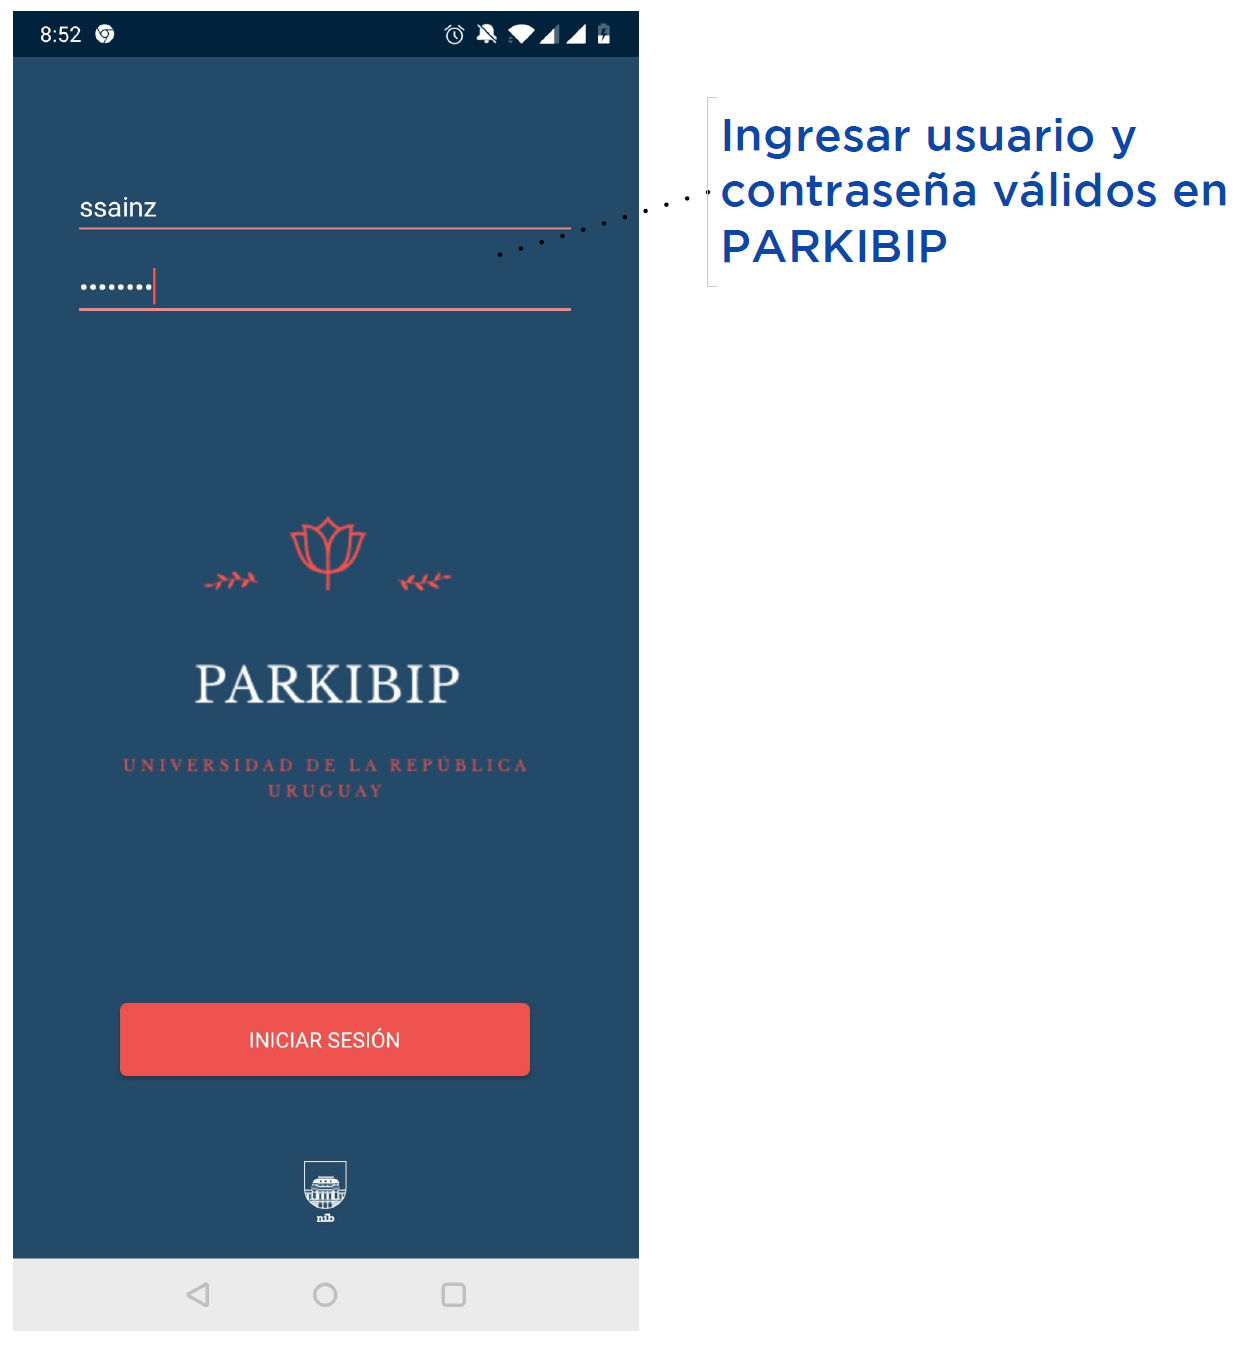
\includegraphics[height=8cm]{TESIS/imagenes/user-manual/manual-login.PNG}
 \caption{Proceso de autenticación y autorización del Usuario. Se requieren los campos nombre de usuario y contraseña.}
 \label{fig:}
\end{figure}

\section{Pantalla inicial y menú de navegación}

Una vez iniciada la sesión, mediante el proceso de autenticación y autorizaciones, se muestra la pantalla inicial de PARKIBIP -ver Fig. \ref{fig:manual-home}-. Siendo ésta una de las principales, ya que es el punto de partida para la ejecución de sesiones de rehabilitación.

\newpage

\begin{figure}[H]
 \centering
 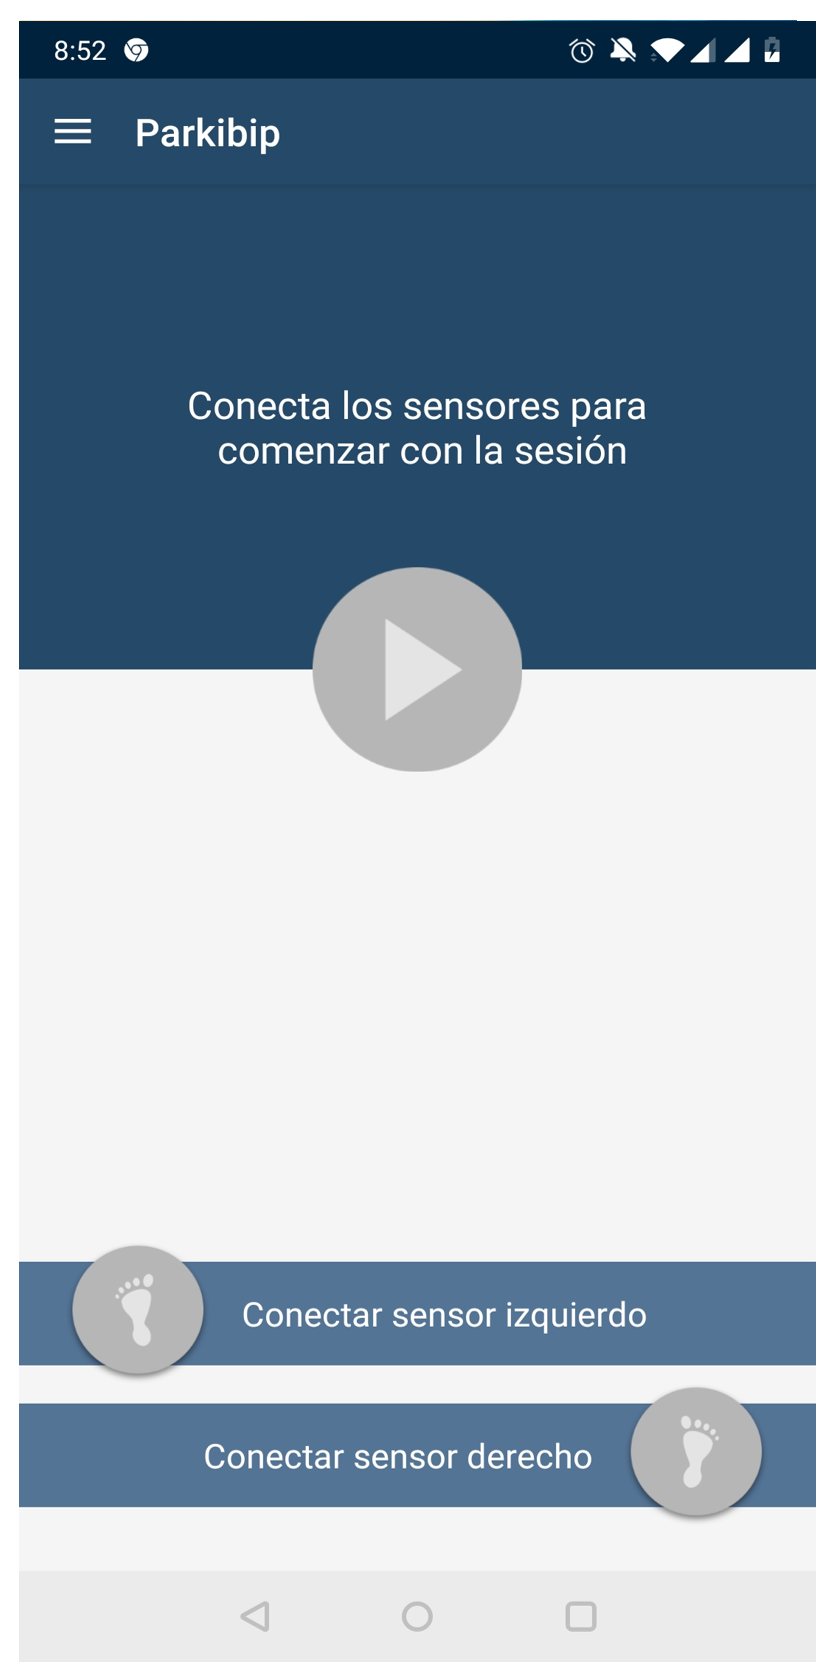
\includegraphics[height=8cm]{TESIS/imagenes/user-manual/manual-home.PNG}
 \caption{Pantalla inicial de PARKIBIP. Dicha pantalla, permite configurar dispositivos IMU e iniciar una sesión de rehabilitación PARKIBIP.}
 \label{fig:manual-home}
\end{figure}

A su vez, la pantalla de inicio, posee un componente moderno de interfaz de usuario. Se trata de un panel lateral que contiene diversas opciones de navegación, y que permanece oculto por defecto en PARKIBIP, tal como se aprecia en la figura previa. Para acceder a esta funcionalidad, basta con deslizar horizontalmente el dedo desde el lateral izquierdo al móvil. Dentro de las opciones de navegación -ver Fig. \ref{fig:manual-navigation}-, se encuentran: (i) Inicio, (ii) Historial de sesiones, (iii) Perfiles de usuarios, (iv) Configuración, (v) Cierre de sesión.

Asimismo, para el Usuario logueado, el sistema distingue su Rol Terapeuta/Paciente, auto-genera una imagen y adjunta el email.

\newpage

\begin{figure}[H]
 \centering
 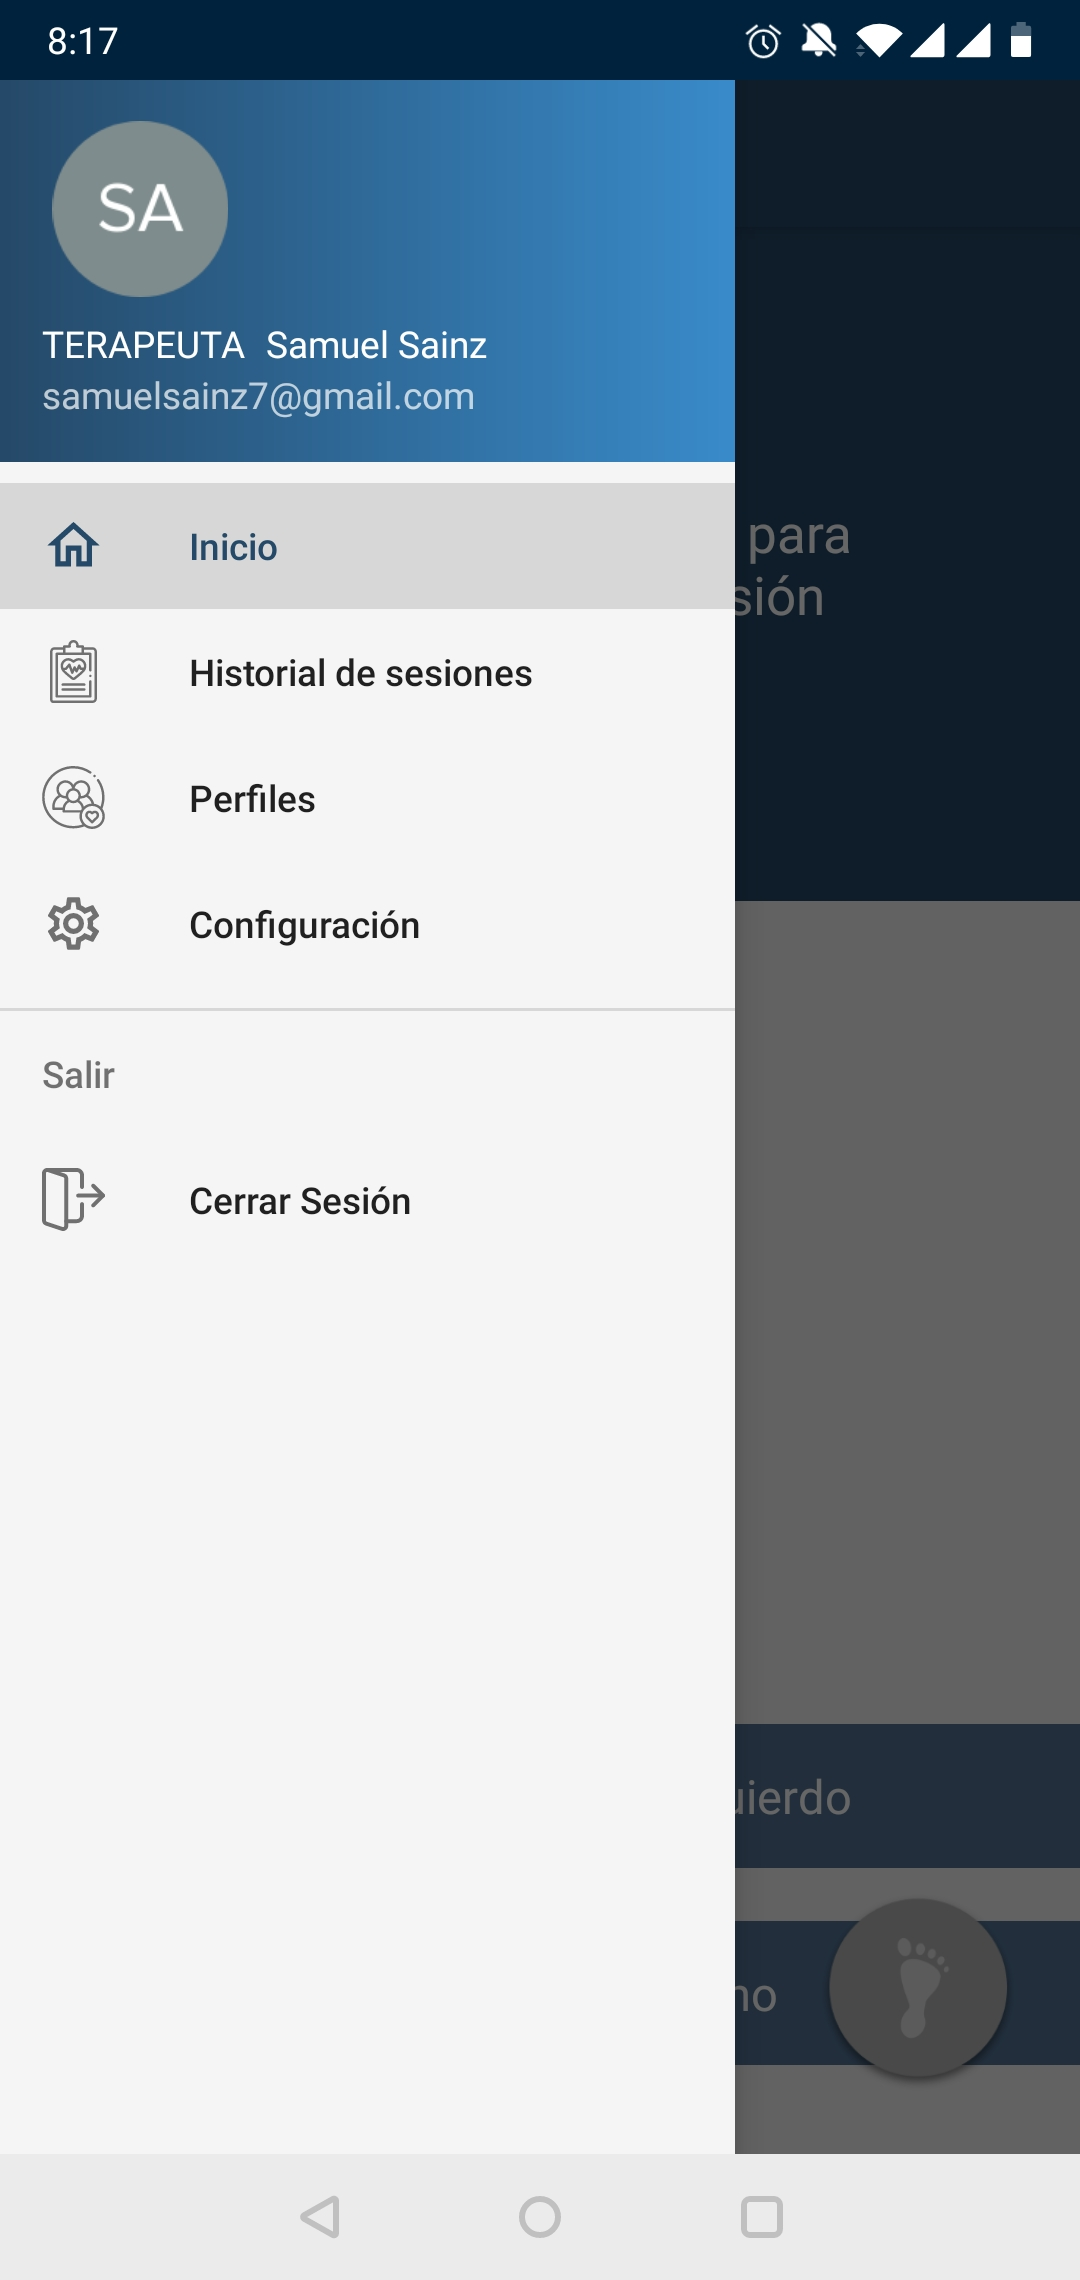
\includegraphics[height=8cm]{TESIS/imagenes/user-manual/manual-navigation.JPG}
 \caption{Panel lateral de navegación. Contiene diversas opciones para navegar a través de los distintos módulos de PARKIBIP.}
 \label{fig:manual-navigation}
\end{figure}

\section{Conexión de IMU}

El objetivo de PARKIBIP, es realizar sesiones de rehabilitación mediante dispositivos IMU. Entonces, es necesario configurarlos adecuadamente. Para ello, se requiere que el modulo de bluetooth del móvil este activado.

Ya con bluetooth y en la pantalla inicial, presionando uno de los botones inferiores -con icono de Pie- comienza el proceso de configuración de un dispositivo para dicho pie. Automáticamente el sistema comienza un escaneo de dispositivos IMU en la cercanía, y despliega un listado de dispositivos encontrados -tal como se aprecia en al Fig. \ref{fig:manual-search}-. Para cada IMU se muestra su identificador MAC, el tipo de dispositivo y la intensidad de la señal del mismo.

\newpage

\begin{figure}[H]
 \centering
 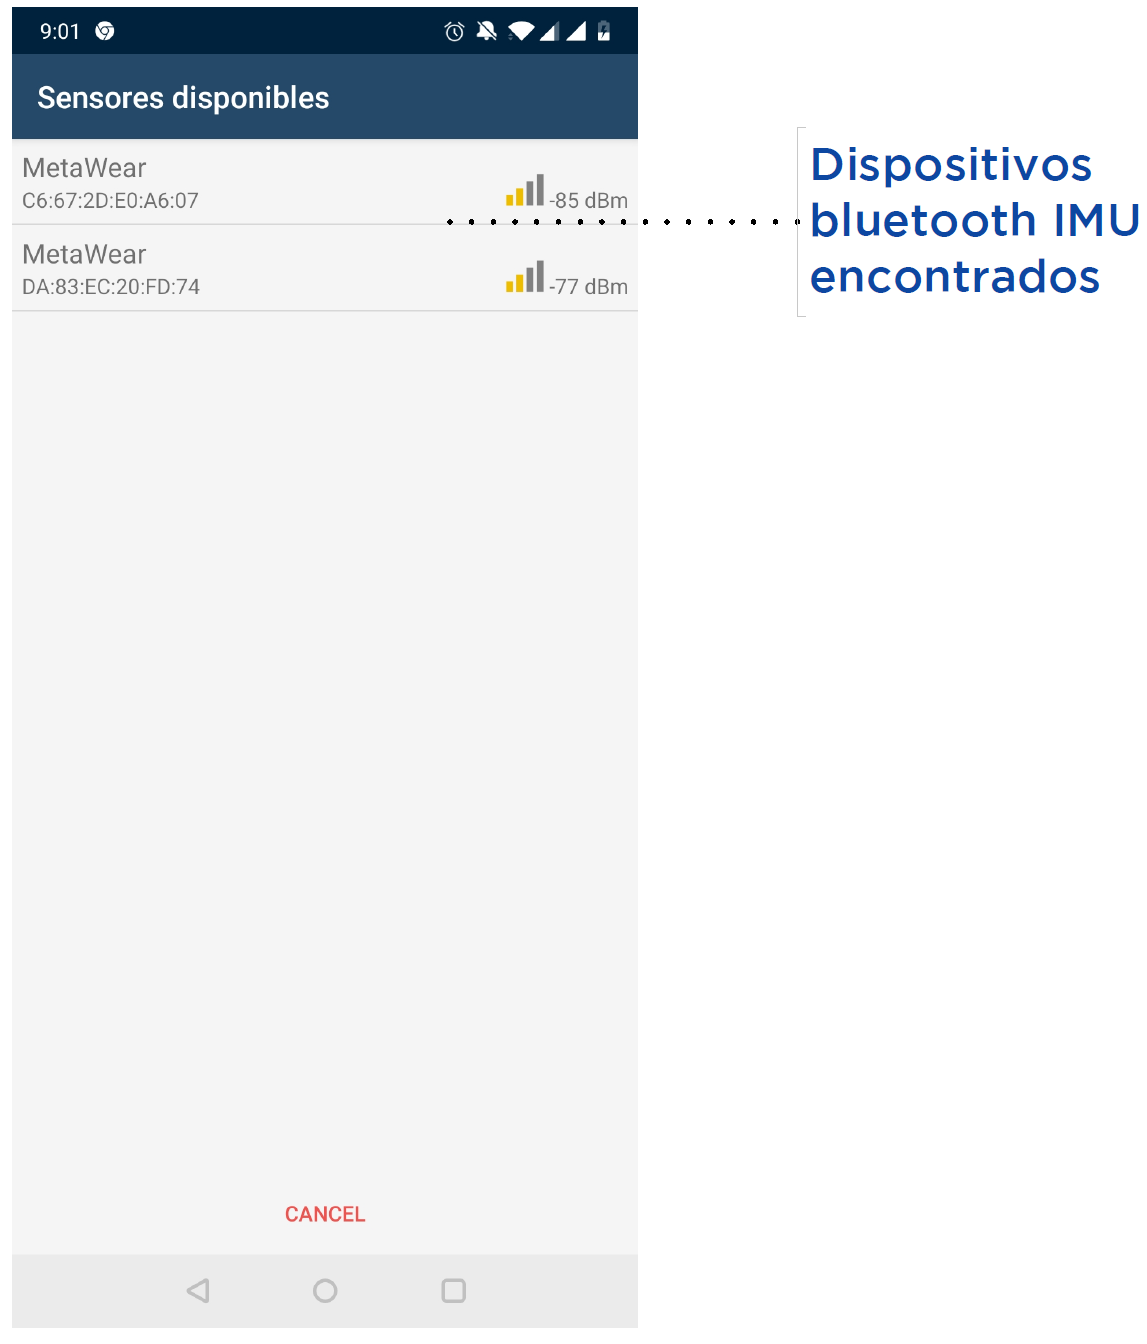
\includegraphics[height=8cm]{TESIS/imagenes/user-manual/manual-search.PNG}
 \caption{Escaneo de dispositivos IMU. Previa activación del modulo bluetooth, expone un listado de IMU en la cercania. Para cada uno muestra su identificador MAC, el tipo de IMU y la intensidad de la señal.}
 \label{fig:manual-search}
\end{figure}

Al seleccionar un IMU dentro de la lista resultante del escaneo, PARKIBIP establece las configuraciones necesarias y se conecta al dispositivo inercial. La figura Fig. \ref{fig:manual-imu-config} expone el éxito de la conexión pintando el botón con el color azul. 

Sumamente importante, PARKIBIP identifica al Pie/IMU con un color en la aplicación, en la imagen rojo, y es el mismo color que comienza a parpadear en el IMU mediante una luz LED.

\newpage

\begin{figure}[H]
 \centering
 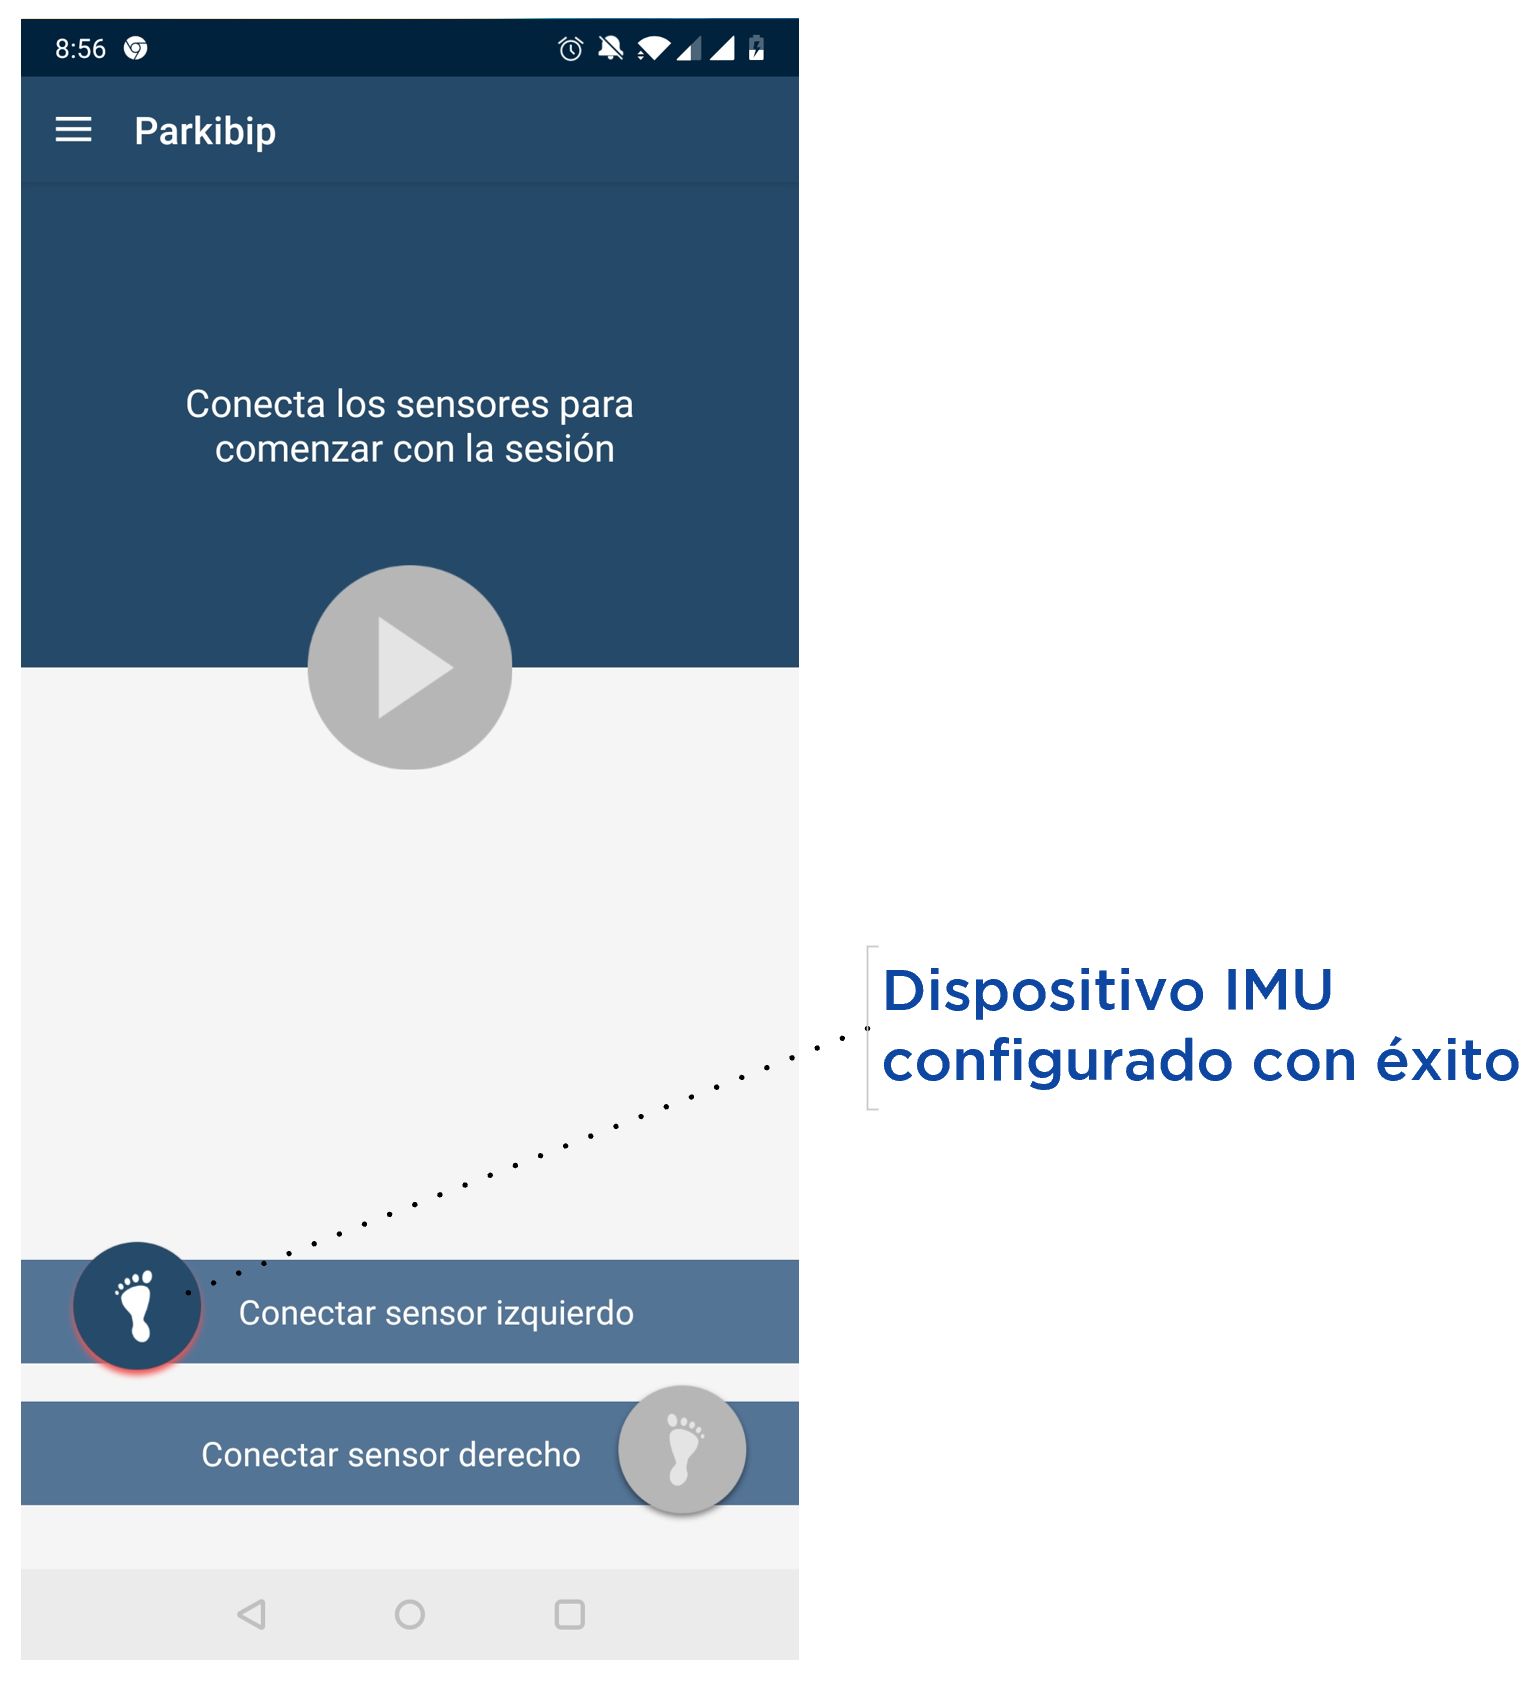
\includegraphics[height=8cm]{TESIS/imagenes/user-manual/manual-imu-config.PNG}
 \caption{Conexión exitosa del IMU asociado al pie izquierdo -botón coloreado de azul-. PARKIBIP identifica al Pie/IMU con un color en la aplicación, en la imagen rojo. Es el mismo color que comienza a parpadear en el IMU mediante su luz LED.}
 \label{fig:manual-imu-config}
\end{figure}

Configurados ambos dispositivos IMU, el sistema habilita el botón que inicia una sesión de rehabilitación PARKIBIP -coloreado con Verde-.

En la figura Fig. \ref{fig:manual-ready}, se aprecia que ambos botones se encuentra en azul, las luces LED del IMU sincronizadas a los colores de los contornos de los botones, y el botón central es puesto en verde.

\newpage

\begin{figure}[H]
 \centering
 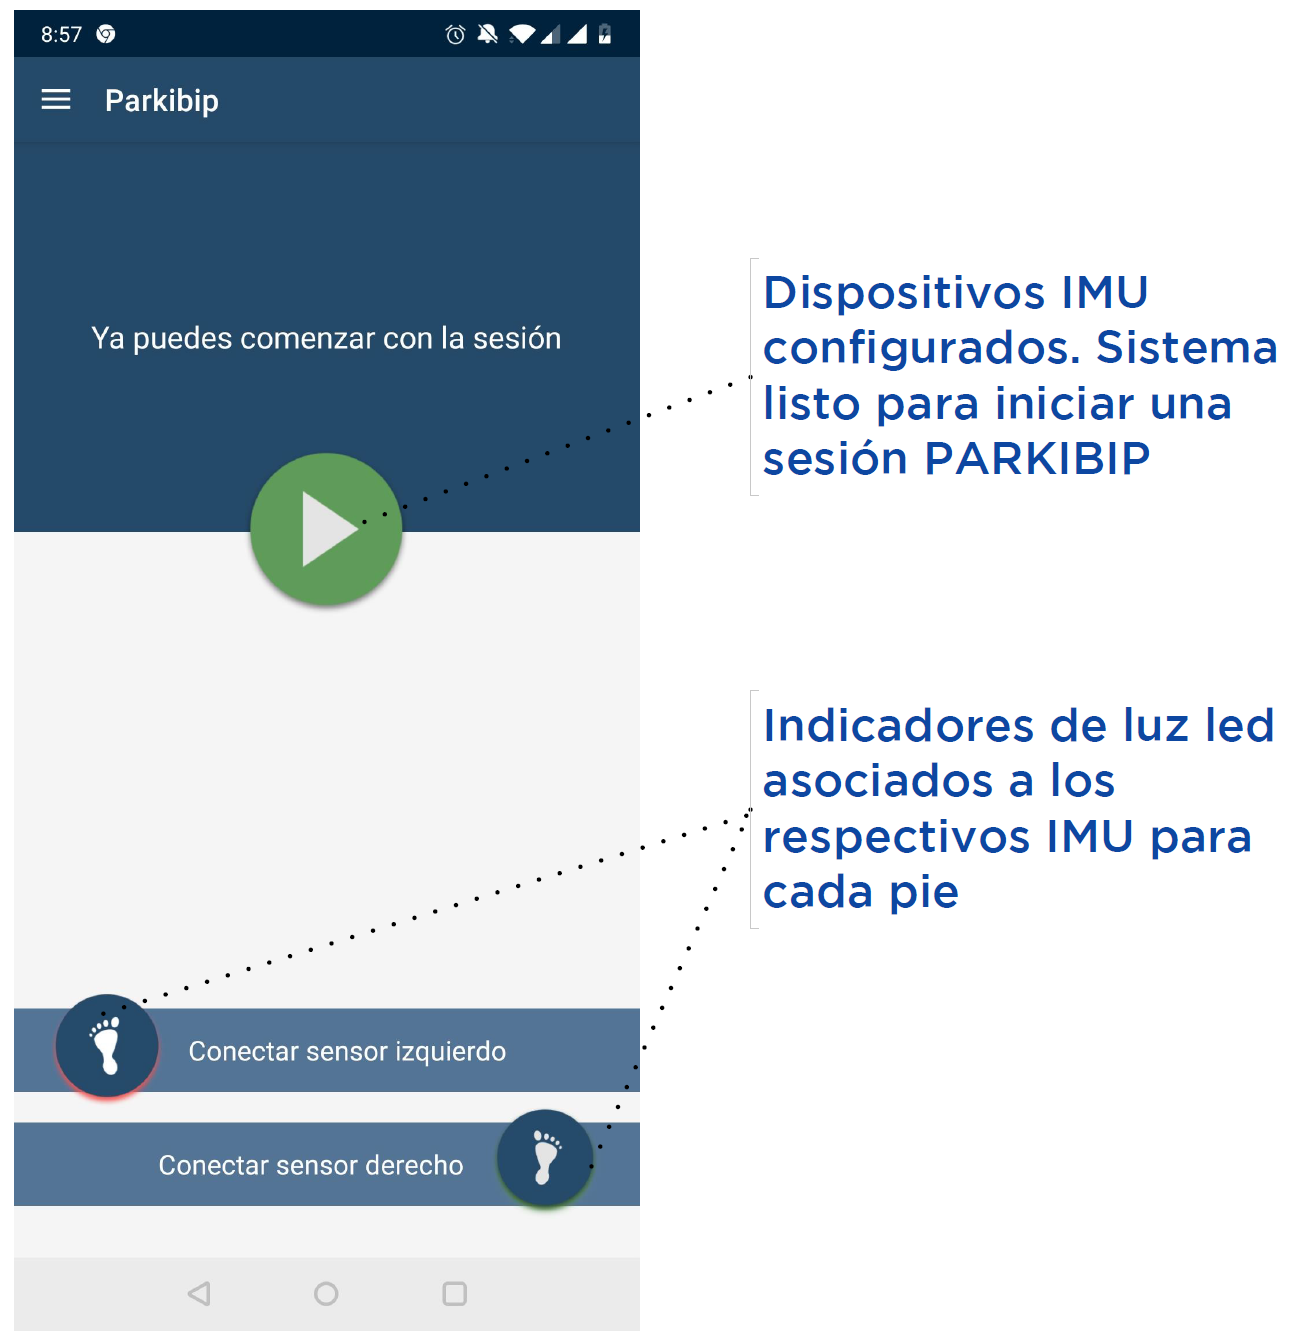
\includegraphics[height=8cm]{TESIS/imagenes/user-manual/manual-ready.PNG}
 \caption{Configuración de los IMU exitosa. Ambos botones se encuentra en azul, las luces LED del IMU sincronizadas a los colores de los contornos de los botones, y el botón central es puesto en verde. PARKIBIP se encuentra listo para comenzar una sesión de rehabilitación.}
 \label{fig:manual-ready}
\end{figure}

\section{Sesión activa de rehabilitación PARKIBIP}

Configurados los dispositivos IMU y presionando el botón que comienza una sesión de rehabilitación, PARKIBIP redirige al usuario a la pantalla esencial del sistema: Sesión Activa. La figura Fig. \ref{fig:manual-active-session} permite visualizar un ejemplo -aleatorio- en tiempo real de sesión PARKIBIP.

\newpage

\begin{figure}[H]
 \centering
 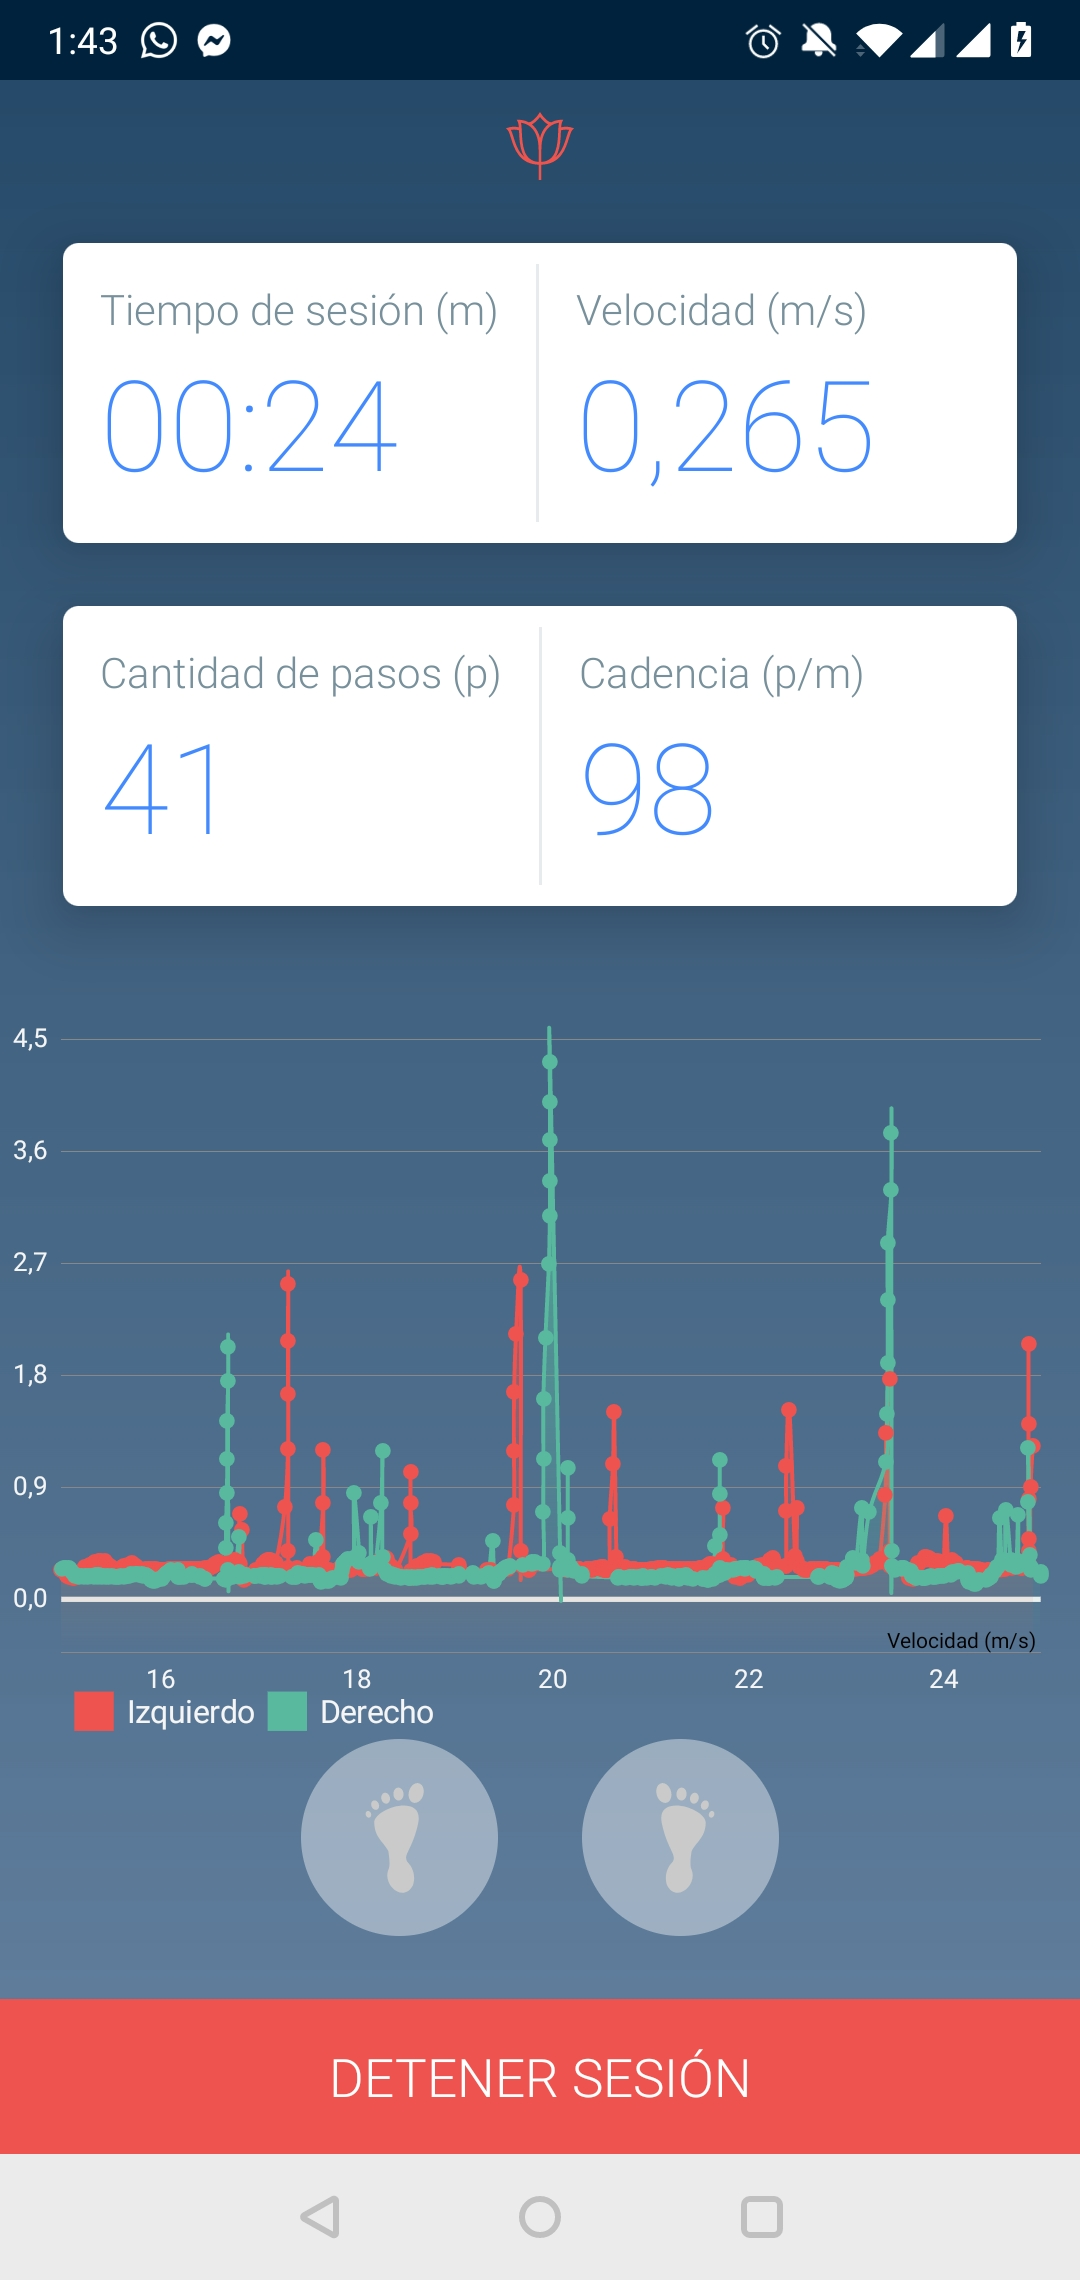
\includegraphics[height=8cm]{TESIS/imagenes/user-manual/manual-active-session.JPG}
 \caption{Pantalla de una Sesión Activa PARKIBIP. El sistema reacciona en tiempo real a la marcha del paciente en rehabilitación. Dispara estímulos externos -vibración y/o sonido- y computa los parámetros espacio-temporales.}
 \label{fig:manual-active-session}
\end{figure}

Tal como se puede apreciar, el sistema reacciona en tiempo real a la marcha del paciente en rehabilitación, mediante el envío de estímulos externos -vibración y/o sonido- y el cómputo de parámetros espacio-temporales. Así, medición a medición, la interfaz de usuario comienza a transitar por distintos valores fruto del procesamiento de PARKIBIP.

\section{Resumen general y detallado}

Finalizada una sesión de rehabilitación PARKIBIP, se podrá evaluar empíricamente la marcha del paciente en cuestión. Así, el sistema redirecciona al usuario a un síntesis, denominada ``Resumen general'' y ``Resumen detallado'' -ver Fig. \ref{fig:manual-resume}-. 

Dentro de la vista general, el sistema presenta el comportamiento de la marcha en términos de valores de parámetros espacio-temporales. Luego, en la vista detallada, se propone un análisis gráfico del comportamiento.  

\begin{figure}[H]
 \centering
 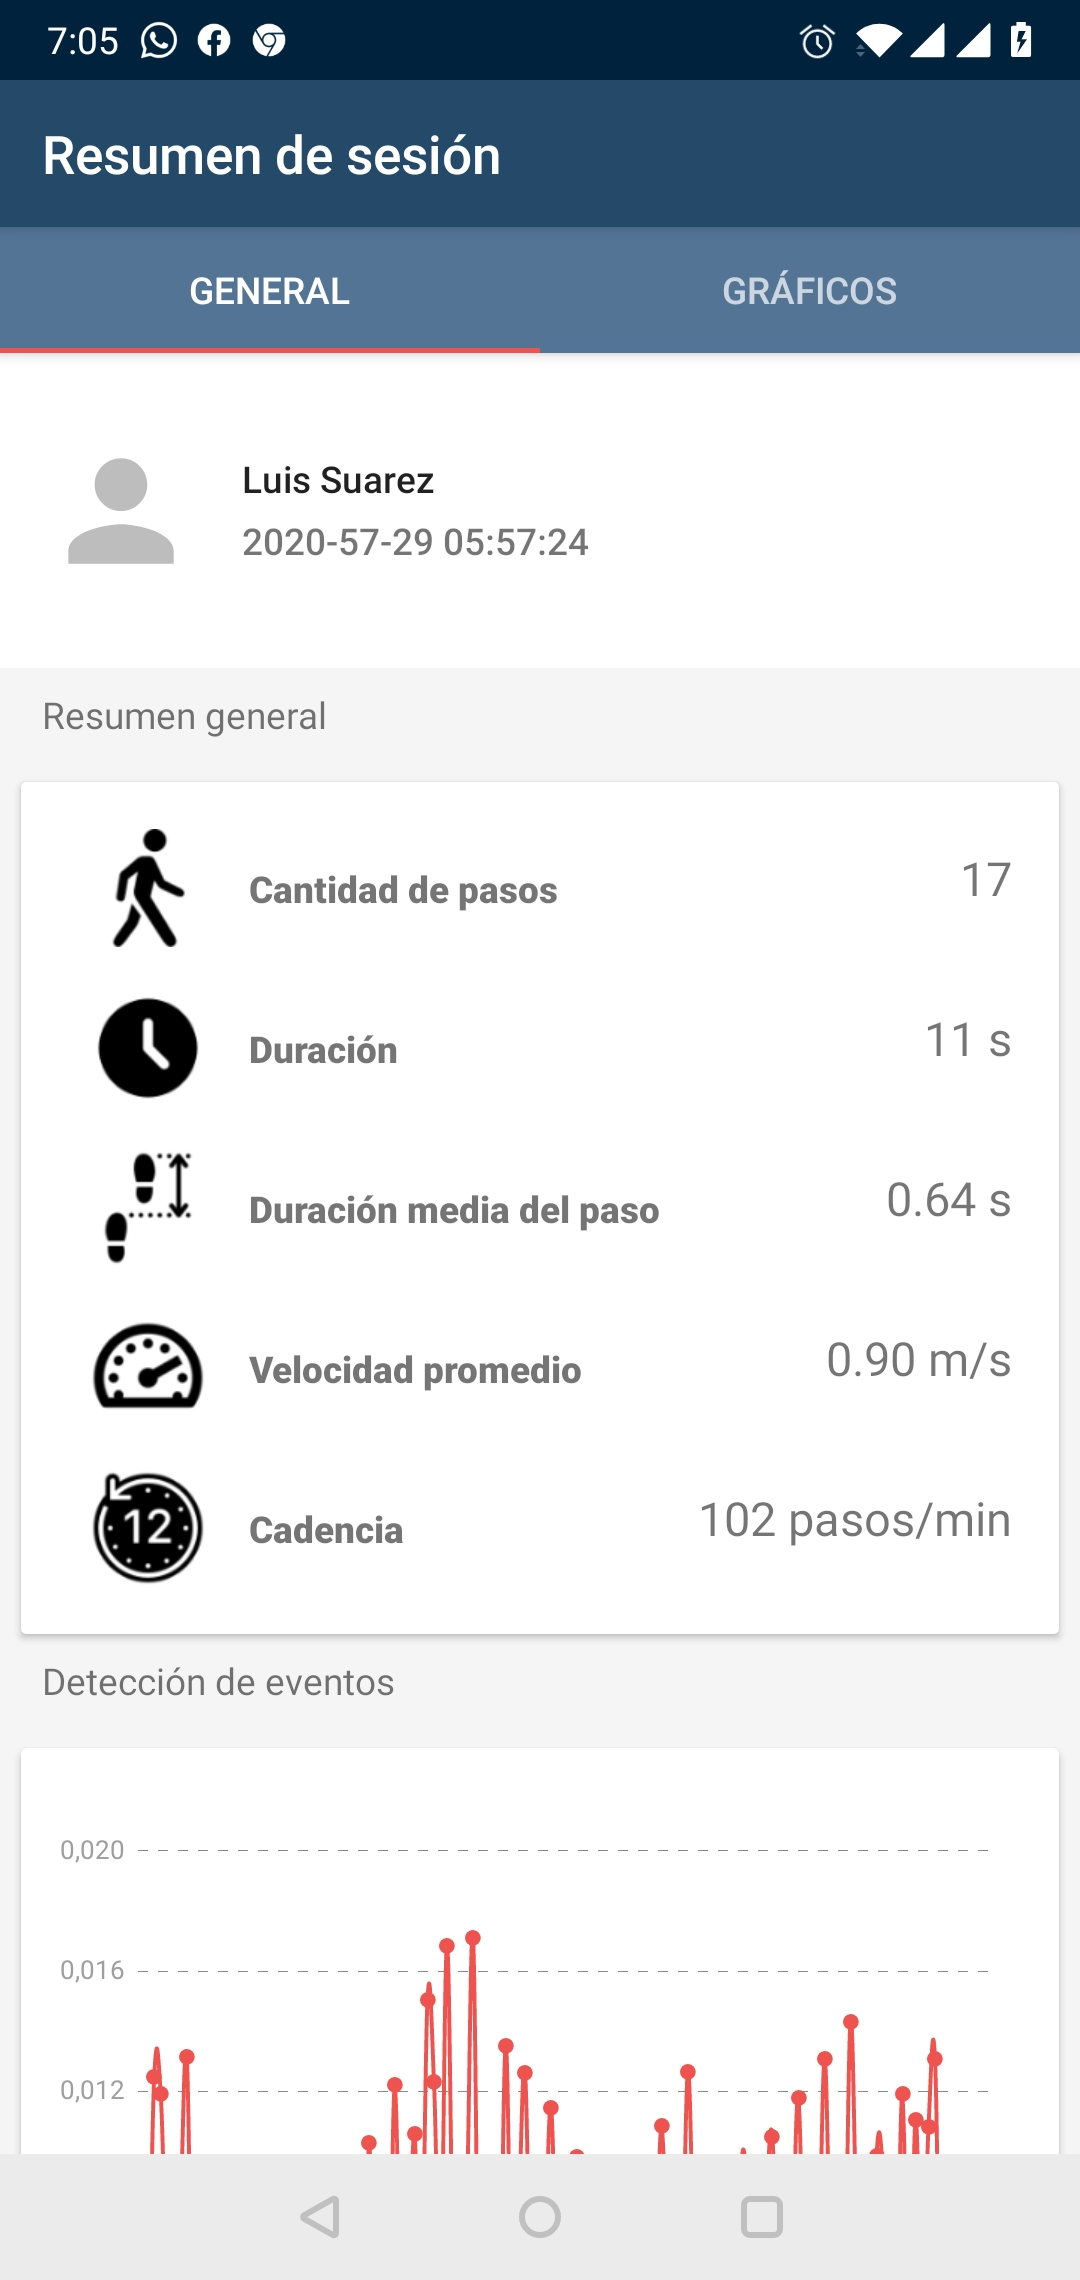
\includegraphics[height=8cm]{TESIS/imagenes/user-manual/manual-resume.JPG}
 \caption{Resumen general y detallado de una sesión. Se presenta el comportamiento de la marcha en términos de valores de parámetros espacio-temporales y de forma gráfica.}
 \label{fig:manual-resume}
\end{figure}

\section{Historial de sesiones}

Desde el panel lateral y mediante la opción de navegación ``Historial de sesiones'', es posible acceder a las distintas sesiones de rehabilitación. Como se puede apreciar en la figura Fig. \ref{fig:manual-history}, se muestra un listado de sesiones ordenadas cronológicamente con su correspondiente fecha y paciente evaluado. Además, en la barra lateral, es posible buscar y filtrar las distintas sesiones por nombre/documento del paciente o fecha de realización. En caso de querer mas información, se puede seleccionar una sesión y navegar a su resumen.

\newpage

\begin{figure}[H]
 \centering
 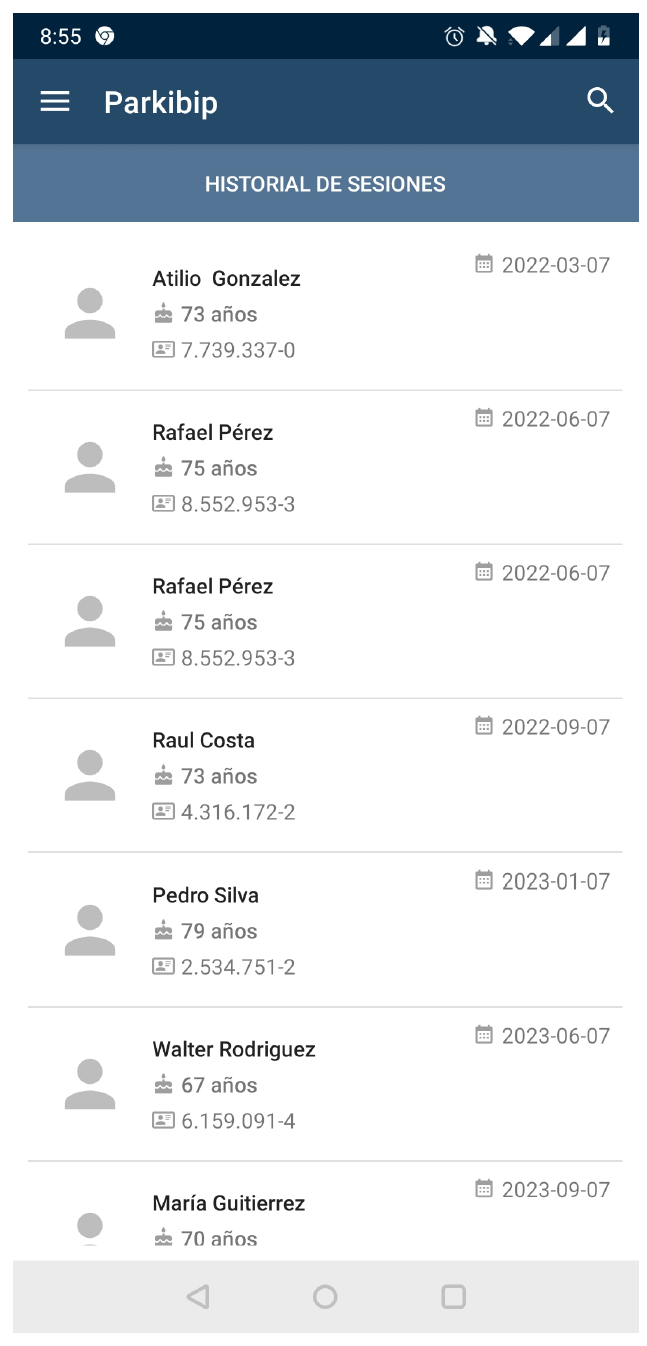
\includegraphics[height=8cm]{TESIS/imagenes/user-manual/manual-history.PNG}
 \caption{Historial de sesiones. Ordenadas cronológicamente con su correspondiente fecha de realización y paciente evaluado. Permite acceder a su resumen mediante su selección.}
 \label{fig:manual-history}
\end{figure}

\section{Usuario y Pacientes}

A partir de la opción ``Perfiles'', en el panel de navegación, es posible visualizar: (i) Información descriptiva del usuario que inicio sesión (i.e. logueado), (ii) Listado de pacientes -en caso de ser un terapeuta-, (iii) Paciente activo para futuras sesiones de rehabilitación.

Dentro de las características del Usuario logueado, el sistema distingue el Rol Terapeuta/Paciente.

Por otro lado, el sistema habilita la selección de un paciente dentro del listado para efectuarle sesiones de rehabilitación con PARKIBIP.

Por último, para lograr mayor celeridad, mediante el menú superior es posible buscar y filtrar el listado de paciente.
\newpage

\begin{figure}[H]
 \centering
 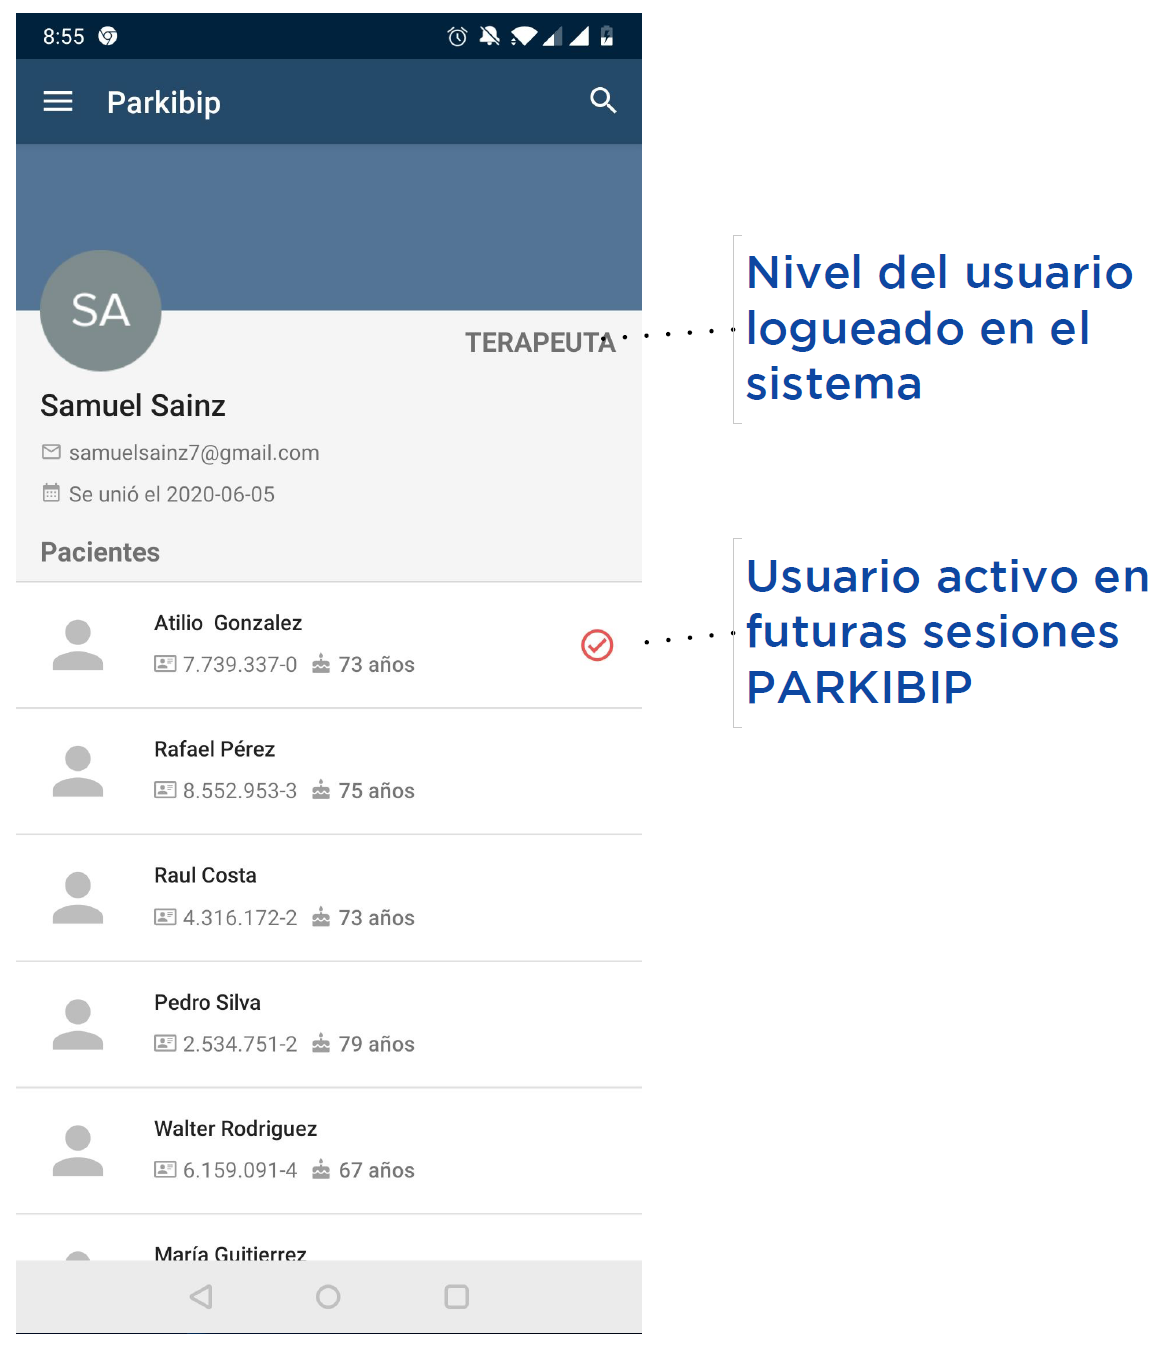
\includegraphics[height=8cm]{TESIS/imagenes/user-manual/manual-users.PNG}
 \caption{Visualización de perfiles de usuarios. Funcionalidades: (i) Ver información descriptiva del usuario logueado, (ii) Ver el listado de pacientes -en caso de ser un terapeuta-, (iii) Seleccionar el paciente activo para futuras sesiones de rehabilitación.}
 \label{fig:manual-users}
\end{figure}

\section{Configuración de métodos y parámetros}

PARKIBIP es una aplicación de ajuste experimental. Es decir, el Terapeuta que evalúa al paciente -previa capacitación técnica-, podrá ajustar los parámetros según las necesidades del paciente en cuestión.

Por lo tanto, PARKIBIP, habilita a modificar los parámetros globales y calibrados por defecto -ver Fig. \ref{fig:manual-config}-. 

\newpage

\begin{figure}[H]
 \centering
 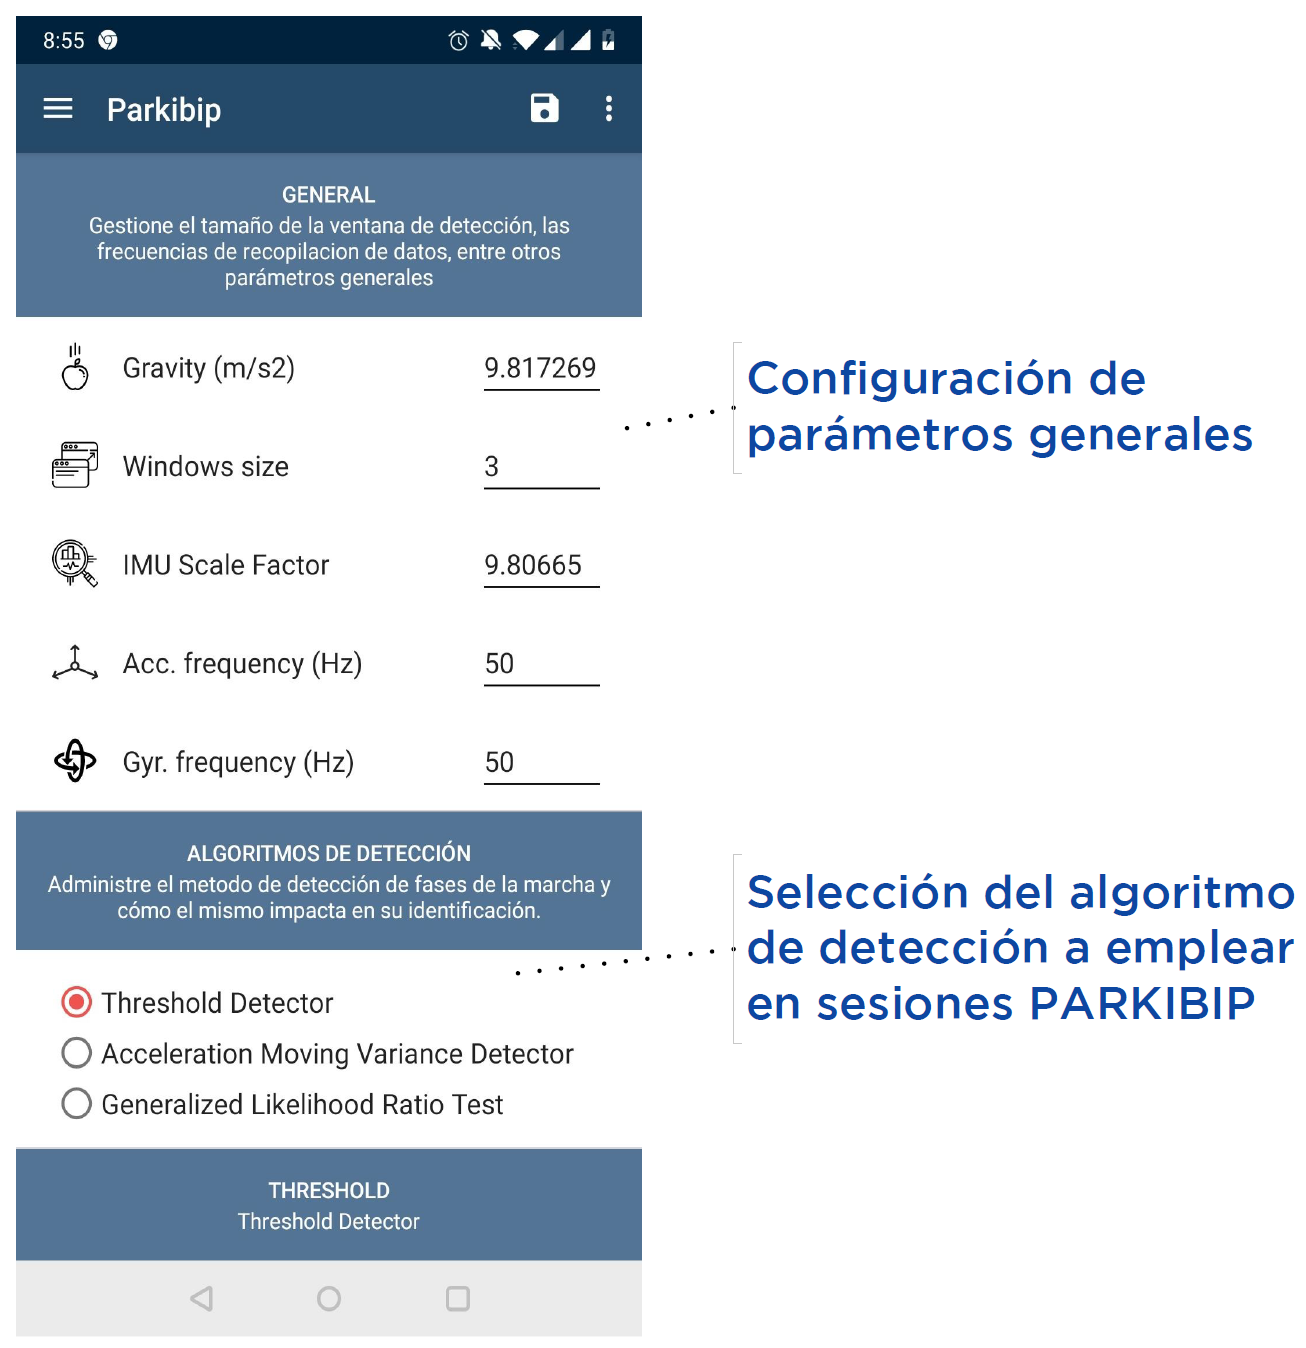
\includegraphics[height=8cm]{TESIS/imagenes/user-manual/manual-config.PNG}
 \caption{Configuración de parámetros y selección del algoritmo de detección. PARKIBIP habilita al usuario a modificar parámetros generales y específicos de los métodos.}
 \label{fig:manual-config}
\end{figure}

Además, podrá experimentar distintos algoritmos de detección de fases de la marcha mediante su selección en formato de grupo de opciones, así como también configurar sus distintos parámetros particulares -ver Fig. \ref{fig:manual-config2}-. 
\begin{figure}[H]
 \centering
 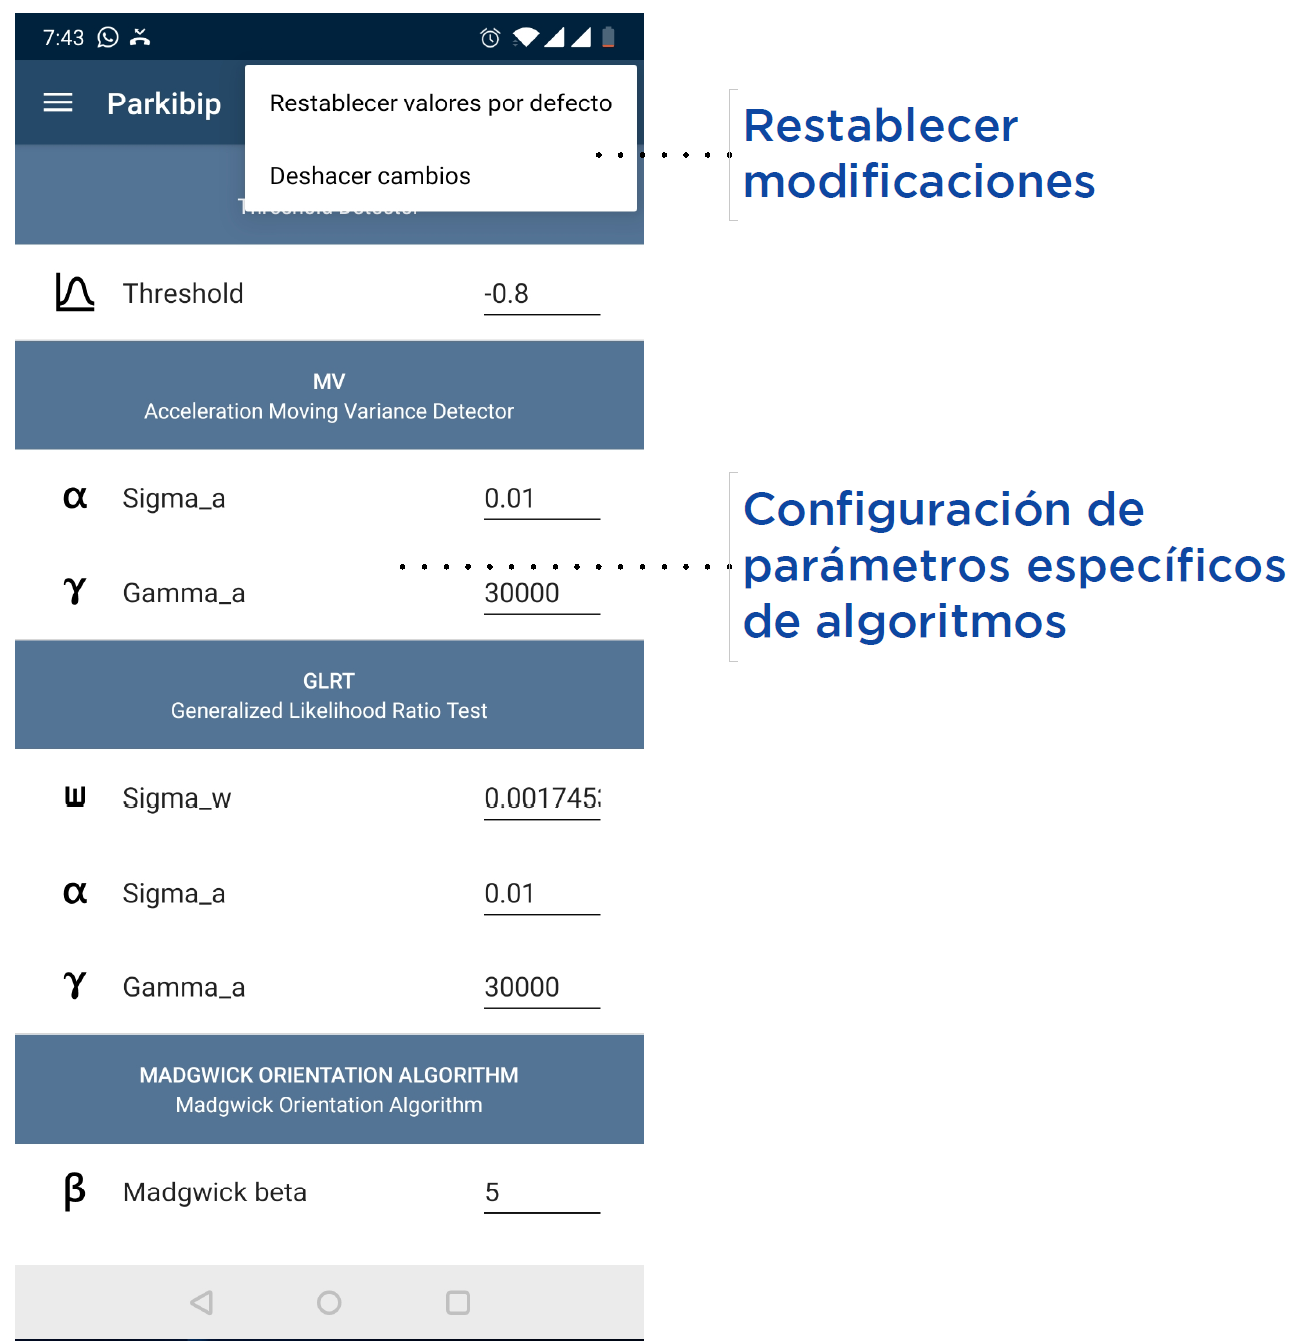
\includegraphics[height=8cm]{TESIS/imagenes/user-manual/manual-config2.PNG}
 \caption{Restauración de valores. PARKIBIP permite restablecer a valores de fabrica, así como descartar cambios efectuados.}
 \label{fig:manual-config2}
\end{figure}

Presionando el botón guardar, del menú superior, los cambios son establecidos.

Por ultimo, pero no menos importante, PARKIBIP viene calibrado con las mejores configuraciones, así que se habilitan las funciones en el menú superior: (i) restablecer a valores de fabrica y (ii) descartar cambios.
